

%% AAPT Physics Bowl Exams Questions
%%----------------------------------------


%% this section contains 33 problems


%% PhysicsBowl 2015
%%----------------------------------------


%% PhysicsBowl 2014
%%----------------------------------------
\element{aapt-A4}{ %% Bowl-A4
\begin{question}{bowl-2014-q09}
    Which one of the following quantities is not a scalar quantity?
    \begin{multicols}{3}
    \begin{choices}
      \correctchoice{Force}
        \wrongchoice{Energy}
        \wrongchoice{Mass}
        \wrongchoice{Speed}
        \wrongchoice{Pressure}
    \end{choices}
    \end{multicols}
\end{question}
}

\element{aapt}{ %% Bowl-A4
\begin{question}{bowl-2014-q11}
    A crate gains \SI{36.0}{\joule} of kinetic energy while its speed is increased from \SI{2.00}{\meter\per\second} to \SI{4.00}{\meter\per\second}.
    Which one of the following choices best represents the mass of the crate?
    \begin{multicols}{3}
    \begin{choices}
        \wrongchoice{\SI{36.0}{\kilo\gram}}
        \wrongchoice{\SI{18.0}{\kilo\gram}}
      \correctchoice{\SI{6.0}{\kilo\gram}}
        \wrongchoice{\SI{3.0}{\kilo\gram}}
        \wrongchoice{\SI{1.5}{\kilo\gram}}
    \end{choices}
    \end{multicols}
\end{question}
}

\element{aapt}{ %% Bowl-A3
\begin{question}{bowl-2014-q13}
    Which one of the following scientists is most associated with the following statement:
        ``For small displacements of an object from equilibrium, there is a restoring force that is proportional to the displacement''?
    \begin{multicols}{2}
    \begin{choices}
        \wrongchoice{Albert Einstein}
      \correctchoice{Robert Hooke}
        \wrongchoice{Christiaan Huygens}
        \wrongchoice{Johannes Kepler}
        \wrongchoice{Heinrich Lenz}
    \end{choices}
    \end{multicols}
\end{question}
}

\element{aapt}{ %% Bowl-A4
\begin{question}{bowl-2014-q31}
    A toy crane exerts an upward force and delivers a useful power output of \SI{0.10}{\watt} to raise a block vertically at a constant speed.
    At what constant speed will this crane raise a \SI{0.20}{\kilo\gram} block?
    \begin{multicols}{3}
    \begin{choices}
        \wrongchoice{\SI{0.01}{\meter\per\second}}
        \wrongchoice{\SI{0.02}{\meter\per\second}}
      \correctchoice{\SI{0.05}{\meter\per\second}}
        \wrongchoice{\SI{0.20}{\meter\per\second}}
        \wrongchoice{\SI{0.50}{\meter\per\second}}
    \end{choices}
    \end{multicols}
\end{question}
}

\element{aapt}{ %% Bowl-A4
\begin{question}{bowl-2014-q32}
    Planck's constant is multiplied by the speed of light.
    The resulting value then is divided by three meters.
    This final value has the units of which one of the following quantities?
    \begin{multicols}{2}
    \begin{choices}
        \wrongchoice{Force}
        \wrongchoice{Linear Momentum}
        \wrongchoice{Speed}
        \wrongchoice{Frequency}
      \correctchoice{Energy}
    \end{choices}
    \end{multicols}
\end{question}
}


%% PhysicsBowl 2013
%%----------------------------------------


%% PhysicsBowl 2012
%%----------------------------------------
\element{aapt}{ %% Bowl-A4
\begin{question}{bowl-2012-q16}
    A constant force $F=\SI{50}{\newton}$ (as shown in the figure)
        is applied for the \SI{6.0}{\meter} motion of the box
        upward along the incline.
    \begin{center}
    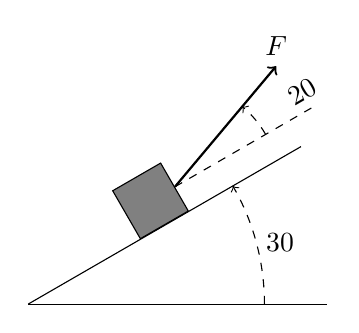
\begin{tikzpicture}
        \draw (0,0) -- ++ (30:4);
        \draw (0,0) -- (0:3.8);
        \draw[dashed,->] (0:3) arc (0:30:3) node[pos=0.5,anchor=west] {\ang{30}};
        \node[draw,rotate=30,anchor=south,fill=white!50!black,rectangle,minimum size=2em] (A) at (30:2) {};
        \draw[dashed] (A.east) -- ++ (30:2) node[anchor=south,rotate=30] {\ang{20}};
        \draw[dashed,->] (A.east) ++ (30:1.33) arc (30:50:1.33);
        \draw[thick,->] (A.east) -- ++ (50:2) node[anchor=south] {$F$};
    \end{tikzpicture}
    \end{center}
    The mass of the block is $M=\SI{15}{\kilo\gram}$.
    Which one of the following choices best represents
        the work done by the force $F$ on the box for the motion?
    \begin{multicols}{3}
    \begin{choices}
        \wrongchoice{\SI{300}{\joule}}
      \correctchoice{\SI{282}{\joule}}
        \wrongchoice{\SI{260}{\joule}}
        \wrongchoice{\SI{193}{\joule}}
        \wrongchoice{\SI{150}{\joule}}
    \end{choices}
    \end{multicols}
\end{question}
}


\element{aapt}{ %% Bowl-A4
\begin{question}{bowl-2012-q18}
    A \SI{1.00}{\kilo\gram} object is released from rest
        near the surface of the Earth.
    The gravitational force acting on the \SI{1.00}{\kilo\gram}
        object by the Earth does \SI{10.0}{\joule} of work on
        the object as it falls \SI{1.00}{\meter} to the ground.
    Which one of the the following choices best represents the
        amount of work done by the gravitational force acting
        on the Earth by the \SI{1.00}{\kilo\gram} object during
        the fall?
    \begin{multicols}{2}
    \begin{choices}
      \correctchoice{\SI{0.0}{\joule}}
        \wrongchoice{\SI{-10.0}{\joule}}
        \wrongchoice{\SI{10.0}{\joule}}
        \wrongchoice{\SI{-5.86e25}{\joule}}
        \wrongchoice{\SI{5.86e25}{\joule}}
    \end{choices}
    \end{multicols}
\end{question}
}

\element{aapt}{ %% Bowl-A4
\begin{question}{bowl-2012-q19}
    The magnitude of the linear momentum of a \SI{4.00}{\kilo\gram}
        point mass is changed from \SI{6.00}{\kilo\gram\meter\per\second}
        to \SI{14.0}{\kilo\gram\meter\per\second} in a time interval
        of \SI{6.00}{\second}.
    What is the change in the kinetic energy of the mass during
        this time interval?
    \begin{multicols}{3}
    \begin{choices}
        \wrongchoice{\SI{8.0}{\joule}}
        \wrongchoice{\SI{10.0}{\joule}}
        \wrongchoice{\SI{16.0}{\joule}}
      \correctchoice{\SI{20.0}{\joule}}
        \wrongchoice{\SI{32.0}{\joule}}
    \end{choices}
    \end{multicols}
\end{question}
}


%% PhysicsBowl 2011
%%----------------------------------------
\element{aapt}{ %% Bowl-A4
\begin{question}{bowl-2011-q36}
    For the inclined plane shown,
        a force of \SI{150}{\newton} applied parallel to the incline's surface is needed to pull the object of mass $M=\SI{10.0}{\kilo\gram}$ along the entire length of the incline's surface at a constant speed.
    \begin{center}
    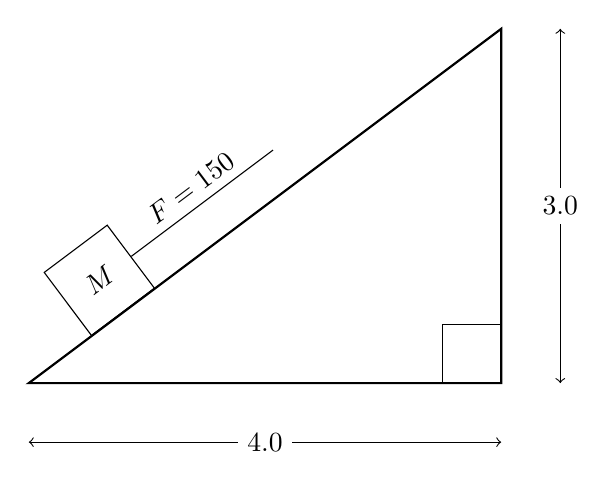
\begin{tikzpicture}[scale=1.5]
        %% 3,4,5, triangle
        \draw[thick] (0,0) -- (4,0) -- (4,3) -- cycle;
        \draw (3.5,0) -- (3.5,0.5) -- (4,0.5);
        %% lengths
        \draw[<->] (0,-0.5) -- (4,-0.5) node[pos=0.5,anchor=center,fill=white] {\SI{4.0}{\meter}};
        \draw[<->] (4.5,0) -- (4.5,3) node[pos=0.5,anchor=center,fill=white] {\SI{3.0}{\meter}};
        %% bot
        \node[draw,minimum size=1cm,anchor=south,rotate=36.86] (M) at (36.86:1) {$M$};
        \draw (M.east) -- ++(36.86:1.5) node[pos=0.5,anchor=south,rotate=36.86] {$F=\SI{150}{\newton}$};
    \end{tikzpicture}
    \end{center}
    What is the actual mechanical advantage (AMA) for this scenario?
    \begin{multicols}{3}
    \begin{choices}
      \correctchoice{$\dfrac{2}{3}$}
        \wrongchoice{$\dfrac{3}{2}$}
        \wrongchoice{$\dfrac{2}{5}$}
        \wrongchoice{$\dfrac{3}{5}$}
        \wrongchoice{$\dfrac{5}{3}$}
    \end{choices}
    \end{multicols}
\end{question}
}

\element{aapt}{ %% Bowl-A4
\begin{question}{bowl-2011-q37}
    Two blocks sit on a horizontal frictionless surface connected to an ideal spring.
    \begin{center}
    \begin{tikzpicture}
        %% floor
        \draw (-3.5,0) -- (3.5,0);
        \node[anchor=north,minimum width=7cm,pattern=north east lines] at (0,0) {};
        %% 2M block
        \node[draw,rounded corners=0.5ex,minimum size=1.5cm,fill=white!90!black,anchor=south] (A) at (-1.5,0) {$2M$};
        %% M block
        \node[draw,rounded corners=0.5ex,minimum size=1.2cm,fill=white!90!black,anchor=south] (B) at (+2,0) {$M$};
        %% spring
        \draw[decoration={aspect=0.2,segment length=2.0mm,amplitude=2mm,coil},decorate] (B.west) -- ++(180:2.15);
        %% string
        \draw[thick] (B.north) -- ++(180:2.75) node[pos=0.6,anchor=south] {string};
    \end{tikzpicture}
    \end{center}
    Initially everything is at rest and there is a string compressing the mass-spring system from equilibrium.
    At some time after the string is cut,
        the block of mass $2M$ reaches its maximum kinetic energy $K$.
    What maximum kinetic energy does the block of mass $M$ attain in terms of $K$?
    \begin{multicols}{3}
    \begin{choices}
        \wrongchoice{$\dfrac{1}{4}K$}
        \wrongchoice{$\dfrac{1}{2}K$}
        \wrongchoice{$K$}
      \correctchoice{$2K$}
        \wrongchoice{$4K$}
    \end{choices}
    \end{multicols}
\end{question}
}


%% PhysicsBowl 2010
%%----------------------------------------
\element{aapt}{ %% Bowl-A4
\begin{question}{bowl-2010-q02}
    Which of the following is \emph{not} a vector quantity?
    \begin{multicols}{2}
    \begin{choices}
        \wrongchoice{Acceleration}
        \wrongchoice{Average Velocity}
        \wrongchoice{Linear Momentum}
      \correctchoice{Potential Energy}
        \wrongchoice{Force}
    \end{choices}
    \end{multicols}
\end{question}
}


%% PhysicsBowl 2009
%%----------------------------------------
\element{aapt}{ %% Bowl-A4
\begin{question}{bowl-2009-q05}
    At an instant of time, a block of mass \SI{0.50}{\kilo\gram}
        has position of \SI{3.0}{\meter}, a speed of
        \SI{4.0}{\meter\per\second}, and acceleration of
        \SI{1.0}{\meter\per\second\squared}.
    What is the block's kinetic energy at this instant?
    \begin{multicols}{3}
    \begin{choices}
        \wrongchoice{\SI{1.0}{\joule}}
        \wrongchoice{\SI{1.5}{\joule}}
        \wrongchoice{\SI{2.0}{\joule}}
      \correctchoice{\SI{4.0}{\joule}}
        \wrongchoice{\SI{8.0}{\joule}}
    \end{choices}
    \end{multicols}
\end{question}
}


%% PhysicsBowl 2008
%%----------------------------------------
\element{aapt}{ %% Bowl-A4
\begin{question}{bowl-2008-q48}
    A block of mass $M$ on a horizontal surface is connected to the end of a massless spring of spring constant $k$.
    The block is pulled a distance $x$ from equilibrium and when released from rest, the block moves toward equilibrium.
    \begin{center}
    \begin{tikzpicture}
        %% Surface
        \node[anchor=north,fill,pattern=north east lines,minimum width=6cm, minimum height=0.05cm] at (-3,0) {};
        \node[anchor=west,fill,pattern=north east lines,minimum width=0.05cm, minimum height=2.25cm] at (0,0.875) {};
        \draw (0,2) -- (0,0) -- (-6,0);
        %% Mass
        \node[fill=white!90!black,draw,rectangle,rounded corners=1ex,minimum size=1.5cm,anchor=south] (M) at (-5.00,0) {$M$};
        \draw[dashed] (M.north) -- ++(90:1);
        \draw[dashed] (-3,2.5) -- ++(270:1.2);
        %% spring
        \draw[decoration={aspect=0.2,segment length=2.0mm,amplitude=2mm,coil},decorate] (0,0.75) -- (M.east) node[pos=0.5,anchor=south,yshift=3mm] {$k$};
        %% Displacement
        \draw[<->] (-5,2) -- (-3,2) node[pos=0.5,anchor=south] {$x$};
    \end{tikzpicture}
    \end{center}
    What minimum coefficient of kinetic friction between the surface and the block would prevent the block from returning to equilibrium with non-zero speed?
    \begin{multicols}{3}
    \begin{choices}
        \wrongchoice{$\dfrac{kx^2}{2Mg}$}
        \wrongchoice{$\dfrac{kx}{Mg}$}
      \correctchoice{$\dfrac{kx}{2Mg}$}
        \wrongchoice{$\dfrac{Mg}{2kx}$}
        \wrongchoice{$\dfrac{k}{4Mgx}$}
    \end{choices}
    \end{multicols}
\end{question}
}


%% PhysicsBowl 2007
%%----------------------------------------
\element{aapt}{ %% Bowl-A4
\begin{question}{bowl-2007-q07}
    A mass connected to a string swings back and forth as a pendulum with snapshots of the motion seen in the figure.
    \begin{center}
    \begin{tikzpicture}
        %% Ceiling
        \node[anchor=south,fill,pattern=north east lines,minimum width=4cm, minimum height=0.05cm] at (0,0) {};
        \draw (-2,0) -- (2,0);
        %% Pendulums
        \node[circle,draw,fill=white!90!black] (A) at (210:3) {$A$};
        \node[circle,draw,fill=white!70!black] (B) at (240:3) {$B$};
        \node[circle,draw,fill=white!50!black] (C) at (270:3) {$C$};
        \node[circle,draw,fill=white!70!black] (D) at (300:3) {$D$};
        \node[circle,draw,fill=white!90!black] (E) at (330:3) {$E$};
        %% Strings
        \draw[dashed] (0,0) -- (A);
        \draw[dashed] (0,0) -- (B);
        \draw (0,0) -- (C);
        \draw[dashed] (0,0) -- (D);
        \draw[dashed] (0,0) -- (E);
    \end{tikzpicture}
    \end{center}
    Ignore the friction in the system.
    Which of the following statements about the pendulum-Earth system is correct?
    \begin{choices}
      \correctchoice{The total mechanical energy in the system is constant.}
        \wrongchoice{The total mechanical energy in the system is maximum at $B$.}
        \wrongchoice{The potential energy at $A$ and $C$ are equal.}
        \wrongchoice{The kinetic energy at $C$ and $D$ are equal.}
        \wrongchoice{The kinetic energy at $C$ and $E$ are equal.}
        %\wrongchoice{The kinetic energy at $E$ equals the kinetic energy at $C$.}
    \end{choices}
\end{question}
}

\element{aapt}{ %% Bowl-A4
\begin{question}{bowl-2007-q15}
    %% Questions 15 and 16 refer to this situation.
    Two identical mass objects are launched with the same speed from the same starting location.
    Object 1 is launched at an angle of \ang{30} above the horizontal while Object 2 is launched at an angle of \ang{60} above the horizontal.
    Ignore air resistance and consider the flight of each object from launch until it returns to the same launch height above the ground.
    %% start question
    Which object returns to the starting height with the greatest speed?
    \begin{choices}
        \wrongchoice{Object 1 since it keeps a lower trajectory.}
        \wrongchoice{Object 2 since it is in the air for a longer time.}
        \wrongchoice{Object 2 since there is more work done on the object during flight.}
      \correctchoice{The speed are the same.}
        \wrongchoice{It cannot be determined without more information.}
    \end{choices}
\end{question}
}

\element{aapt}{ %% Bowl-A4
\begin{question}{bowl-2007-q22}
    A mass $m$ is pulled outward until the string of length $L$ to which it is attached makes a \ang{90} angle with the vertical.
    The mass is released from rest and swings through a circular arc.
    What is the tension in the string when the mass swings through the bottom of the arc?
    \begin{multicols}{2}
    \begin{choices}
        \wrongchoice{$0$}
        \wrongchoice{$mg$}
        \wrongchoice{$2mg$}
      \correctchoice{$3mg$}
        \wrongchoice{It cannot be determined}
    \end{choices}
    \end{multicols}
\end{question}
}


%% PhysicsBowl 2006
%%----------------------------------------
\element{aapt}{ %% Bowl-A4
\begin{question}{bowl-2006-q09}
    A deliveryman moves 10 cartons from the sidewalk, along a \SI{10}{\meter}
        ramp to a loading dock, which is \SI{1.5}{\meter} above the sidewalk.
    %% NOTE: diagram, but not necessary
    If each carton has a mass of \SI{25}{\kilo\gram},
        what is the total work done by the deliveryman on the cartons to move them to the loading dock?
    \begin{multicols}{2}
    \begin{choices}
        \wrongchoice{\SI{2 500}{\joule}}
      \correctchoice{\SI{3 750}{\joule}}
        \wrongchoice{\SI{10 000}{\joule}}
        \wrongchoice{\SI{25 000}{\joule}}
        \wrongchoice{\SI{37 500}{\joule}}
    \end{choices}
    \end{multicols}
\end{question}
}

\element{aapt}{ %% Bowl-A4
\begin{question}{bowl-2006-q19}
    A \SI{60.0}{\kilo\gram} ball of clay is tossed vertically in the air
        with an initial speed of \SI{4.60}{\meter\per\second}.
    Ignoring air resistance,
        what is the change in its potential energy when it reaches its highest point?
    \begin{multicols}{3}
    \begin{choices}
        \wrongchoice{\SI{0}{\joule}}
        \wrongchoice{\SI{45}{\joule}}
        \wrongchoice{\SI{280}{\joule}}
      \correctchoice{\SI{635}{\joule}}
        \wrongchoice{\SI{2700}{\joule}}
    \end{choices}
    \end{multicols}
\end{question}
}

\element{aapt}{ %% Bowl-A4
\begin{question}{bowl-2006-q20}
    A boy jumps from rest straight upward from a flat,
        stationary concrete surface.
    The boy, of mass $M$, leaves the concrete surface with speed $v$
        and his center of mass rises a distance $d$ to the highest point of the motion.
    How much physical work did the average normal force of contact ($N$)
        between the boy's feet and the concrete do on the boy?
    \begin{multicols}{3}
    \begin{choices}
        \wrongchoice{$Nd$}
        \wrongchoice{$\dfrac{Mv^2}{2}$}
        \wrongchoice{$\dfrac{Nd}{2}$}
        \wrongchoice{$Mgd$}
      \correctchoice{zero}
    \end{choices}
    \end{multicols}
\end{question}
}

\element{aapt}{ %% Bowl-A4
\begin{question}{bowl-2006-q32}
    The kilowatt hour (\si{\kilo\watt\hour}) is a unit of:
    \begin{multicols}{2}
    \begin{choices}
        \wrongchoice{Power.}
      \correctchoice{Energy.}
        \wrongchoice{Force.}
        \wrongchoice{Impulse.}
        \wrongchoice{Voltage.}
    \end{choices}
    \end{multicols}
\end{question}
}



%% PhysicsBowl 2005
%%----------------------------------------
\element{aapt}{ %% Bowl-A4
\begin{question}{bowl-2005-q05}
    A box of old textbooks is on the middle shelf in the
        bookroom \SI{1.3}{\meter} from the floor.
    If the janitor relocates the box to the shelf that is
        \SI{2.6}{\meter} from the floor, how much work
        does he do on the box.
    The box has a mass of \SI{10.0}{\kilo\gram}.
    \begin{multicols}{3}
    \begin{choices}
        \wrongchoice{\SI{13.0}{\joule}}
        \wrongchoice{\SI{26.0}{\joule}}
        \wrongchoice{\SI{52.0}{\joule}}
      \correctchoice{\SI{130}{\joule}}
        \wrongchoice{\SI{260}{\joule}}
    \end{choices}
    \end{multicols}
\end{question}
}

\element{aapt}{ %% Bowl-A4
\begin{question}{bowl-2005-q28}
    A mass, $M$, is at rest on a frictionless surface,
        connected to an ideal horizontal spring that is unstretched.
    A person extends the spring \SI{30}{\centi\meter} from
        equilibrium and holds it at this location by
        applying a \SI{10}{\newton} force.
    The spring is brought back to equilibrium and the mass
        connected to it is now doubled to $2M$.
    If the spring is extended back \SI{30}{\centi\meter} from
        equilibrium, what is the necessary force applied
        by the person to hold the mass stationary there?
    \begin{multicols}{2}
    \begin{choices}
        \wrongchoice{\SI{20.0}{\newton}}
        \wrongchoice{\SI{14.1}{\newton}}
      \correctchoice{\SI{10.0}{\newton}}
        \wrongchoice{\SI{7.07}{\newton}}
        \wrongchoice{\SI{5.00}{\newton}}
    \end{choices}
    \end{multicols}
\end{question}
}

\element{aapt}{ %% Bowl-A4
\begin{question}{bowl-2005-q44}
    A box of mass $m$ is initially at rest on a horizontal surface.
    A constant horizontal force of $\dfrac{mg}{2}$ is applied to the box,
        directed to the right.
    The coefficient of friction of the surface changes with the
        distance pushed as $\mu = \mu_0 x$ where $x$ is the distance
        from the initial location.
    For what distance is the box pushed until it returns to rest?
    \begin{multicols}{3}
    \begin{choices}
        \wrongchoice{$\dfrac{4}{\mu_0}$}
        \wrongchoice{$\dfrac{2}{\mu_0}$}
      \correctchoice{$\dfrac{1}{\mu_0}$}
        \wrongchoice{$\dfrac{1}{2\mu_0}$}
        \wrongchoice{$\dfrac{1}{4\mu_0}$}
    \end{choices}
    \end{multicols}
\end{question}
}



%% PhysicsBowl 2000
%%----------------------------------------
\element{aapt}{ %% Bowl-A4
\begin{question}{bowl-2000-q36}
    A ball is thrown vertically upward with an initial
        velocity $v$ and an initial kinetic energy $E_k$.
    When the ball is half way to the top of its flight,
        it has a velocity of \rule[-0.1pt]{4em}{0.1pt}
        and a kinetic energy of \rule[-0.1pt]{4em}{0.1pt}.
    \begin{multicols}{2}
    \begin{choices}
        \wrongchoice{$\dfrac{v}{2}$, $\dfrac{E_k}{2}$}
      \correctchoice{$\dfrac{v}{\sqrt{2}}$, $\dfrac{E_k}{2}$}
        \wrongchoice{$\dfrac{v}{4}$, $\dfrac{E_k}{2}$}
        \wrongchoice{$\dfrac{v}{2}$, $\dfrac{E_k}{\sqrt{2}}$}
        \wrongchoice{$\dfrac{v}{\sqrt{2}}$, $\dfrac{E_k}{\sqrt{2}}$}
    \end{choices}
    \end{multicols}
\end{question}
}



%% PhysicsBowl 1999
%%----------------------------------------
\element{aapt}{ %% Bowl-A4
\begin{question}{bowl-1999-q10}
    A simple machine can \emph{not} do which of the following:
    \begin{choices}
        \wrongchoice{have a mechanical advantage greater than 1.}
        \wrongchoice{change the direction of the force.}
        \wrongchoice{move the resistance a greater distance than the applied force.}
      \correctchoice{increase the energy put into it.}
        \wrongchoice{produce a force in the resistance which is greater than the applied force.}
    \end{choices}
\end{question}
}

\element{aapt}{ %% Bowl-A4
\begin{question}{bowl-1999-q14}
    A construction laborer holds a \SI{20}{\kilo\gram} sheet
        of wallboard \SI{3}{\meter} above the floor for \SI{4}{\second}.
    During these \SI{4}{\second} how much power was expended
        on the wallboard?
    \begin{multicols}{2}
    \begin{choices}
        \wrongchoice{\SI{2400}{\watt}}
        \wrongchoice{\SI{320}{\watt}}
        \wrongchoice{\SI{27}{\watt}}
        \wrongchoice{\SI{15}{\watt}}
      \correctchoice{None of the provided}
    \end{choices}
    \end{multicols}
\end{question}
}



%% PhysicsBowl 1998
%%----------------------------------------
\element{aapt}{ %% Bowl-A4
\begin{question}{bowl-1998-q01}
    Which of the following is not a vector quantity?
    \begin{multicols}{2}
    \begin{choices}
        \wrongchoice{acceleration}
        \wrongchoice{electric field}
      \correctchoice{energy}
        \wrongchoice{force}
        \wrongchoice{velocity}
    \end{choices}
    \end{multicols}
\end{question}
}


%% PhysicsBowl 1997
%%----------------------------------------
\element{aapt}{ %% Bowl-A4
\begin{question}{bowl-1997-q01}
    A force $F$ directed at an angle of $q$ above the horizontal is used to pull a crate a distance $D$ across a level floor.
    The work done by the force $F$ is:
    \begin{multicols}{2}
    \begin{choices}
        \wrongchoice{$FD$}
      \correctchoice{$FD \cos\theta$}
        \wrongchoice{$FD \sin\theta$}
        \wrongchoice{$mg \sin\theta$}
        \wrongchoice{$mgD \cos\theta$}
    \end{choices}
    \end{multicols}
\end{question}
}

\element{aapt}{ %% Bowl-A4
\begin{question}{bowl-1997-q03}
    A student working on an energy conservation problem has obtained the answer \SI{50}{\joule\second\squared\per\meter\squared}.
    The student has solved for:
    \begin{multicols}{3}
    \begin{choices}
        \wrongchoice{energy}
        \wrongchoice{force}
      \correctchoice{mass}
        \wrongchoice{velocity}
        \wrongchoice{work}
    \end{choices}
    \end{multicols}
\end{question}
}

\element{aapt}{ %% Bowl-A4
\begin{question}{bowl-1997-q10}
    A compressed spring has \SI{16}{\joule} of potential energy.
    What is the maximum speed it can impart to a \SI{2.0}{\kilo\gram} object?
    \begin{multicols}{3}
    \begin{choices}
        \wrongchoice{\SI{2.8}{\meter\per\second}}
      \correctchoice{\SI{4.0}{\meter\per\second}}
        \wrongchoice{\SI{5.6}{\meter\per\second}}
        \wrongchoice{\SI{8.0}{\meter\per\second}}
        \wrongchoice{\SI{16}{\meter\per\second}}
    \end{choices}
    \end{multicols}
\end{question}
}


%% PhysicsBowl 1996
%%----------------------------------------
\element{aapt}{ %% Bowl-A4
\begin{question}{bowl-1996-q20}
    A force of \SI{10}{\newton} stretches a spring that has a spring constant of \SI{20}{\newton\per\meter}.
    The potential energy stored in the spring is:
    \begin{multicols}{3}
    \begin{choices}
      \correctchoice{\SI{2.5}{\joule}}
        \wrongchoice{\SI{5.0}{\joule}}
        \wrongchoice{\SI{10}{\joule}}
        \wrongchoice{\SI{40}{\joule}}
        \wrongchoice{\SI{200}{\joule}}
    \end{choices}
    \end{multicols}
\end{question}
}

\element{aapt}{ %% Bowl-A4
\begin{question}{bowl-1996-q24}
    A \SI{2.0}{\kilo\gram} ball is attached to a \SI{0.80}{\meter} string and whirled in a horizontal circle at a constant speed of \SI{6.0}{\meter\per\second}.
    \begin{center}
    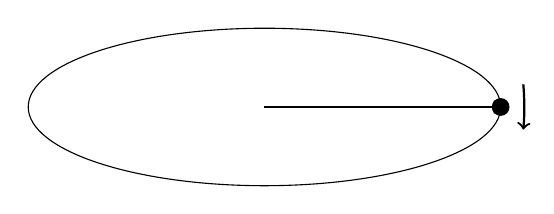
\begin{tikzpicture}
        \draw (0,0) ellipse (3cm and 1cm);
        \draw[thick,->] (0,0) -- (3,0);
        \draw[fill] (3,0) circle (3pt);
        \draw[thick,->] (5:3.3) arc (5:-5:3.3cm);
    \end{tikzpicture}
    \end{center}
    The work done on the ball during each revolution is:
    \begin{multicols}{3}
    \begin{choices}
        \wrongchoice{\SI{450}{\joule}}
        \wrongchoice{\SI{90}{\joule}}
        \wrongchoice{\SI{72}{\joule}}
        \wrongchoice{\SI{16}{\joule}}
      \correctchoice{zero}
    \end{choices}
    \end{multicols}
\end{question}
}

\element{aapt}{ %% Bowl-A4
\begin{question}{bowl-1996-q38}
    A pendulum bob mass $m$ on a cord length $L$ is pulled sideways until the cord makes an angle $\theta$ with the vertical as shown in the figure below.
    \begin{center}
    \begin{tikzpicture}
        %% Ceiling
        \node[anchor=south,fill,pattern=north east lines,minimum width=4cm, minimum height=0.05cm] at (0,0) {};
        \draw (-2,0) -- (2,0);
        %% Min
        \draw[dashed] (0,0) -- (0,-3) node[pos=0.5,anchor=west] {$L$};
        \draw[fill=white] (0,-3) circle (5pt);
        %% Max
        \draw (0,0) -- (225:3);
        \draw[fill] (225:3) circle (5pt);
        %% Vector
        \draw[thick,->] (270:3.5) arc (270:225:3.5);
        \draw (270:0.75) arc (270:225:0.75) node[anchor=north,pos=0.5] {$\theta$};
    \end{tikzpicture}
    \end{center}
    The change in potential energy of the bob during the displacement is:
    \begin{multicols}{2}
    \begin{choices}
      \correctchoice{$mgL \left(1-\cos\theta\right)$}
        \wrongchoice{$mgL \left(1-\sin\theta\right)$}
        \wrongchoice{$mgL \sin\theta$}
        \wrongchoice{$mgL \cos\theta$}
        \wrongchoice{$2mgL \left(1-\sin\theta\right)$}
    \end{choices}
    \end{multicols}
\end{question}
}


%% PhysicsBowl 1995
%%----------------------------------------
\element{aapt}{ %% Bowl-A4
\begin{question}{bowl-1995-q15}
    If the unit for force is $\mathrm{F}$,
        the unit for velocity $\mathrm{V}$,
        and the unit for time $\mathrm{T}$,
        then the unit for energy is:
    \begin{multicols}{3}
    \begin{choices}
      \correctchoice{$\mathrm{FVT}$}
        \wrongchoice{$\dfrac{\mathrm{F}}{\mathrm{T}}$}
        \wrongchoice{$\dfrac{\mathrm{FV}}{\mathrm{T}}$}
        \wrongchoice{$\dfrac{\mathrm{F}}{\mathrm{T}^2}$}
        \wrongchoice{$\dfrac{\mathrm{FV}^2}{\mathrm{T}^2}$}
    \end{choices}
    \end{multicols}
\end{question}
}

\element{aapt}{ %% Bowl-A4
\begin{question}{bowl-1995-q17}
    Which is a vector quantity?
    \begin{multicols}{2}
    \begin{choices}
        \wrongchoice{energy}
        \wrongchoice{mass}
      \correctchoice{momentum}
        \wrongchoice{power}
        \wrongchoice{work}
    \end{choices}
    \end{multicols}
\end{question}
}


%% PhysicsBowl 1994
%%----------------------------------------
\element{aapt}{ %% Bowl-A4
\begin{question}{bowl-1994-q05}
    A mass $m$; attached to a horizontal massless spring with spring constant $k$;
        is set into simple harmonic motion.
    \begin{center}
    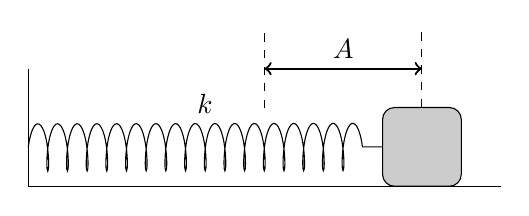
\begin{tikzpicture}
        \draw (0,1.5) -- (0,0) -- (6,0);
        \node[draw,fill=white!80!black,rectangle,rounded corners=1ex,minimum size=1cm,anchor=south] (M) at (5,0) {};
        \draw[decoration={aspect=0.2,segment length=2.5mm,amplitude=3mm,coil},decorate] (0,0.5) -- (M.west) node[pos=0.5,anchor=south,yshift=3mm] {$k$};
        \draw[dashed] (M.north) -- ++(90:1);
        \draw[dashed] (3,1) -- (3,2);
        \draw[thick,<->] (3,1.5) -- (5,1.5) node[anchor=south,pos=0.5] {$A$};
    \end{tikzpicture}
    \end{center}
    Its maximum displacement from its equilibrium position is $A$.
    What is the mass's speed as it passes through its equilibrium position?
    \begin{multicols}{2}
    \begin{choices}
        \wrongchoice{zero}
      \correctchoice{$A\sqrt{\dfrac{k}{m}}$}
        \wrongchoice{$A\sqrt{\dfrac{m}{k}}$}
        \wrongchoice{$\dfrac{1}{A}\sqrt{\dfrac{k}{m}}$}
        \wrongchoice{$\dfrac{1}{A}\sqrt{\dfrac{m}{k}}$}
    \end{choices}
    \end{multicols}
\end{question}
}

\element{aapt}{ %% Bowl-A4
\begin{question}{bowl-1994-q38}
    A force $F$ at an angle $\theta$ above the horizontal is used to pull a heavy
        suitcase of weight $mg$ a distance $d$ along a level floor at constant velocity.
    The coefficient of friction between the floor and the suitcase is $\mu$.
    The work done by the frictional force is:
    \begin{multicols}{2}
    \begin{choices}
      \correctchoice{$-Fd \cos\theta$}
        \wrongchoice{$mgh -Fd \cos\theta$}
        \wrongchoice{$-\mu Fd \cos\theta$}
        \wrongchoice{$-\mu mgd$}
        \wrongchoice{$-\mu mgd \cos\theta$}
    \end{choices}
    \end{multicols}
\end{question}
}


\endinput


